
\section{Contributions to Driftfusion}
	\epigraph{\textit{\enquote{Wow, this is a gold mine!}}}

	\subsection{Introduction}
		During my 3-month stay in Dr.\ Piers R.\ F.\ Barnes and Prof.\ Jenny Nelson groups in Imperial College London, I utilized and expanded a modelling software developed by Dr.\ Phil Calado, Dr.\ Mohammed Azzouzi, Benjamin Hilton, and Piers R.\ F.\ Barnes.
		As the modelling software had already demonstrated a great descriptive power \cite{Belisle2017,Calado2016,Calado2018b}, I implemented a few more characterization techniques with the objective of reproducing and understanding real-world data.
		The impedance spectroscopy simulation is not included here as it has been treated in \cref{ch:impedance}.
		Driftfusion CITE AAAAAAAAAAAAAAUTHORS is a time resolved, one dimensional, drift\hyp{}diffusion modelling platform.
		It takes advantage of Matlab \texttt{pdepe} solver for partial differential equations with boundary conditions in time and one spatial dimension.
		%Solve initial-boundary value problems for parabolic-elliptic PDEs in 1-D.
		Currently, it can simulate the electrostatic potential, and the density of electrons, holes and one ionic specie at specified depths in a multi\hyp{}layered electronic device and at specified time points.
		Even if an heterojunction version of the code is available, I implemented functions for the homojunction (every material has the same bandgap) release, which is much more stable and tested.
		All the described scripts can be obtained from \url{https://github.com/barnesgroupICL/Driftfusion/tree/2018-EIS}.


	\subsection{Additions to the Driftfusion Core}
		\epigraph{$>>$ 0.1 + 0.2 == 0.3\\
			ans =\\
			logical\\
			0}{MATLAB}



\paragraph{\texttt{equilibrate\_minimal} -- Generate a reduced set of solutions at standard conditions}
It's a reduced version of \texttt{equilibrate}. 
Uses analytical initial conditions and runs to equilibrium and steady state, obtaining just the most important solutions
 Takes the parameters from \texttt{pinParams.m} file and tries
 to obtain a steady state solution (as if the device has been left for
 a long period of time). This solution can then be used as accurate
 initial conditions for other simulations, \textsl{e.g.} a JV scan.
 Note that the stabilization time is consistently adjusted to appropriate values for to
 ensure there are numerous mesh points where large gradients in the time
 dimension are present.
 
\textit{Inputs:} optional, struct containing the needed parameters as obtained
     from \texttt{pinParams.m}.
     
\textit{Outputs:} \texttt{sol\_eq} - short circuit, dark, no mobile ionic defects, no \gls{srh};
   \texttt{sol\_i\_eq} - short circuit, dark, mobile ionic defects, no \gls{srh};
   \texttt{sol\_i\_eq\_SR} - short circuit, dark, mobile ionic defects, with \gls{srh};
   \texttt{ssol\_i\_eq} - open circuit, dark, mobile ionic defects, no \gls{srh};
   \texttt{ssol\_i\_eq\_SR} - open circuit, dark, mobile ionic defects, with \gls{srh};
   \texttt{sol\_i\_1S\_SR} - short circuit, 1 sun, mobile ionic defects, with \gls{srh};
   \texttt{ssol\_i\_1S\_SR} - open circuit, 1 sun, mobile ionic defects, with \gls{srh}.

\textit{Requires:} \texttt{pindrift}, \texttt{pinParams}, \texttt{stabilize}.

%\textit{Required by:} 

		\paragraph{\texttt{verify\-Stabilization} -- Verifies if the provided solution has evolved until its steady state}\label{verifyStabilization}
Checks if the solution reached a stabilized (\textsl{i.e.} steady state) status comparing the final time point with a manually specified time point. Beware that this can have false positives when the analysed solution had
 has been run over a time which is so small that the ionic movement did not even start.
 For each variable under study, the comparison integrates over the solution thickness the absolute value of the difference in the profile of this variable at two different times in the solution.
 If this integrated difference is larger than \num{1e-4} times the integrated profile of the same variable at the final time point at which its spatially average value has been subtracted, the solution is considered as not stabilized yet.
 The definition of this last threshold, will cause completely flat profiles to be unsuitable for this check.
 The variables which are employed are: ionic density, electrostatic potential, decimal logarithm of electrons density and decimal logarithm of holes density.
 
\textit{Inputs:} 1) a solution matrix, not the full structure, as contained in
     structures created by \texttt{pindrift};
   2) the time mesh array, as generated by \texttt{meshgen\_t} and included
     in structures created by \texttt{pindrift};
   3) the fraction of final time that can be used as a
     reference. In case of a stabilization, the smaller the stricter the
     check, for example if a solution has been run over \SI{10}{\s}, and the provided fraction is \num{1e-5}, the script will compare the solution at \SI{0.1}{\us} with the final one at \SI{10}{\s}. In case of a periodic time evolution, a specific value
     corresponding to the previous-to last cycle have to be used. The
     value needs to be strictly between 0 and 1.

\textit{Outputs:} a logic (true/false) asserting if the solution in input reached its stability.

%\textit{Requires:} nothing.

\textit{Required by:} 

		\paragraph{\texttt{stabilize} -- Evolves a solution until its steady state}
Simulates the solution increasing the maximum time until when steady state is reached. 
\texttt{verify\-Stabilization} is used for checking the reaching of the steady state.
For all the simulations including transients, the stabilization of the starting solution is of utmost importance.

\textit{Inputs:} 1) a solution structure as created by \texttt{pindrift};
   2) optional boolean, true by default, 
     if true forces the simulation to run at least once, if false the
     stabilization is run just when needed.
     
\textit{Outputs:} a solution structure that reached its steady state.

\textit{Requires:} \texttt{pindrift}, \texttt{verify\-Stabilization}.

\textit{Required by:} 

		\paragraph{\texttt{asymmetricize} -- Break a symmetrical solution}\label{asymmetricize}
		Break a symmetrical solution (a symmetrical solution it's a repeated p-i-n-n-i-p stack, mainly used for simulating open circuit conditions, so that no boundary condition has to be set for the cathode) in two halves. Has the opposite use of the \texttt{symmetricize} function.
		Please note that further stabilization could be required.
		
		\textit{Inputs:} a symmetric structure as created by \texttt{pindrift} using the OC parameter set to 1.
		
		\textit{Outputs:} an asymmetric structure as created by \texttt{pindrift} using the OC
		     parameter set to 0 and applied voltage identical to the open circuit
		     voltage taken from the input symmetric structure.
		     
	\textit{Requires:} \texttt{pindrift}
	
	\textit{Required by:} 

		\paragraph{\texttt{change\-Light} -- Change the illumination intensity of a solution}
		Generate solutions at a new light intensity.
		\textit{Inputs:} 1) a solution structure as created by \texttt{pindrift};
		2) the requested light intensity, zero is not supported as it is
		    much more robust to obtain a dark solution directly from equilibrate;
		3) the initial stabilization time, can be zero for an automatic
		     guess.
		\textit{Outputs:} a solution structure at the new light intensity.
		\textit{Requires:} \texttt{pindrift}, \texttt{stabilize}
			\textit{Required by:} 
			
		\paragraph{\texttt{gen\-Int\-Structs} -- Generates a list of solutions at various light intensities}\label{genIntStructs}
Generates a cell containing structures of solutions at logarithmically spaced light intensities, starting from the one at lower light illumination. Can be used for both symmetrical (for obtaining open circuit solutions) or asymmetrical solutions.

		\textit{Inputs:} 1) a solution struct as created by \texttt{pindrift} in dark conditions, or a logic false for not having the dark; 
		2) highest requested illumination;
		3) lowest requested illumination;
		4) number of illumination requested between the lowest and the highest illumination points, including extrema, except dark;
		5) logical, whether to include the dark solution in the output     structure
		
\textit{Outputs:} 1) a cell containing structures of solutions at various light
     intensities;
2) an array with the voltages present in the solution, which is
     an approximation of the \gls{voc}, getting populated just if the input
     structures were at open circuit;
 3) an array with the currents present in the solutions.
 
\textit{Requires:} \texttt{change\-Light}, \texttt{pindrift}, \texttt{pinana}.

\textit{Required by:} 

		\paragraph{\texttt{gen\-Vapp\-Structs} -- Generates a list of solutions at various applied voltages}\label{genVappStructs}
Generates a cell containing asymmetric structures of solutions at various applied voltages.
Differently from \texttt{gen\-Int\-Structs} case, here the voltage array has to be specified.

\textit{Inputs:} 1) a solution asymmetric struct as created by \texttt{pindrift};
2) an array containing the requested applied voltages list.

\textit{Outputs:} a cell containing structures of solutions at various applied
     voltages, ordered with ascending voltages.
     
\textit{Requires:} \texttt{pindrift}, \texttt{pinana}, \texttt{stabilize}.

\textit{Required by:} 

		\paragraph{\texttt{find\-Optim\-Voc} -- Find the exact \gls{voc} minimizing the current output}
Stabilize an asymmetric solution to the real open circuit voltage
which is the applied voltage where the current is minimized,
starting from the voltage present in the given solution. The suggested
workflow is to stabilize a symmetric solution (so that the charges
profile are close to OC conditions) and break in a half with
\texttt{asymmetricize}.
Differently from \texttt{findVoc}, this version requires MATLAB's Optimization Toolbox.
While the \gls{voc} can be conveniently obtained from the symmetrical solution, in same cases the zero current condition is not matched.
For this reason, the search for an applied voltage that minimizes the residual current can be needed.
		
		\textit{Inputs:} an asymmetric structure as created by \texttt{pindrift}, ideally
    breaking a symmetric solution using \texttt{asymmetricize} function so that
    the starting applied voltage is already close to the real \gls{voc}.
    
\textit{Outputs:} 1) an asymmetric structure as created by \texttt{pindrift} using the OC
     parameter set to 0 and applied voltage identical to the real open
     circuit voltage;
2) the value of the obtained open circuit voltage.

\textit{Requires:} \texttt{pindrift}, \texttt{pinana}, \texttt{stabilize}.

\textit{Required by:} 

		\paragraph{\texttt{gen\-Int\-Structs\-Real\-Voc} -- Generates a list of solutions at various light intensities ensuring open circuit}
		Generates a cell containing structures of asymmetric solutions at various light intensities at an accurate \gls{voc}.
		This script just uses other three scripts: \texttt{gen\-Int\-Structs}, \texttt{find\-Optim\-Voc}
		 and \texttt{asymmetricize}. Both symmetric and asymmetric solutions are supported in input, but the usage of symmetric solutions is strongly encouraged as the \texttt{find\-Optim\-Voc} will start from a condition closer to the \gls{voc}.
		
				\textit{Inputs:} 1) a solution structure as created by \texttt{pindrift} in dark
				     conditions, preferably a symmetric (open circuit) solution;
				2) higher requested illumination;
				3) lower requested illumination;
				4) number of requested illumination points between the lowest and the highest illuminations, including extrema, except dark;
				5) logical, whether to include the dark solution in the output
				     structure.
				
		\textit{Outputs:} 1) cell containing structures of asymmetric solutions at various light
		     intensities with an applied voltage equal to the \gls{voc};
		2) an array with the \gls{voc} values.
		
		\textit{Requires:} \texttt{change\-Light}, \texttt{pindrift}, \texttt{gen\-Int\-Structs},
		   \texttt{asymmetricize}, \texttt{find\-Optim\-Voc}, \texttt{stabilize}.
		   
		\textit{Required by:} 
		
		\paragraph{\texttt{fromSteadyStateStructToTxt} -- Exports stabilized solutions data to text for plotting externally}
		Save the main data from a stabilized solution created by \texttt{pindrift} to text files, using a format easy to import with Origin (from OriginLab).
				\textit{Inputs:} 1) a structure as created by \texttt{pindrift};
				2) a char array to be used as prefix for the saved files names.
%		\textit{Outputs:} none.
%		\textit{Requires:} nothing.
%		\textit{Required by:} 

		\paragraph{\texttt{plot\_charges\_single} -- Plots various density and energy profiles over time}
Plot free charges and ions densities, and energy levels over device thickness and over time.
 This is inspired by Dr.\ Phil Calado's \texttt{pinExtract2.m} but rewritten.
 The created graphics include: profiles of net charge density and 
 comparison with the final profile; conduction and valence bands and 
 quasi-Fermi levels profiles; profiles of total concentration of 
 particles densities and comparison with the final profile, divided 
 per particle type; time evolution of voltage, current and specific 
 particles types in specific positions.

		\textit{Inputs:} 1) a symmetric or asymmetric structure of a solution evolving over time;
		2) optional char array, if provided saves the images in the current directory with the name starting with it.
%\textit{Outputs:} 
%\textit{Requires:} 
%\textit{Required by:} 

		\paragraph{\texttt{examples\_unit\_test} -- Runs unit testing on all the implemented experiments}
Runs various simulations in order to test the functioning of pindrift and many other implemented functions.
Additionally it verifies that the results satisfies some basic checks.
 For profiling the time spent running each function run \texttt{profile on} before running the tests and \texttt{profile viewer} after.
 Using Matlab's Coverage Reports, the unused code can be easily spotted.

%		\textit{Inputs:} 
%\textit{Outputs:} 
\textit{Requires:} \texttt{ideality\_from\_dark\_jVpoints}, \texttt{ideality\_from\_Voc}, \texttt{ISwave\_full\_exec}, \texttt{ISwave\_full\_exec\_nonparallel}, \texttt{equilibrate\_minimal}, \texttt{gen\-Int\-Structs}, \texttt{gen\-Vapp\-Structs}.
%\textit{Required by:} 

%	\subsection{Ideality Factor}
			\paragraph{\texttt{ideality\_from\_Voc} -- Obtains ideality factor from voltage versus illumination intensity relation}\label{dd_ideality}
	As explained in \cpageref{characterization_ideality}, the ideality factor can be obtained relating \gls{voc} to the light intensity.
	%		 data of a device illuminated at various illumination intensities
	
			\textit{Inputs:} a cell containing structures at open circuit and various
	     light intensities. The open circuit can be either obtained from
	     symmetric solutions (from \texttt{gen\-Int\-Structs}) or from asymmetric solutions
	     with applied voltage (from \texttt{gen\-Int\-Structs\-Real\-Voc}).
	
	\textit{Outputs:} the numeric ideality factor.
	
	\textit{Requires:} \texttt{pinana}.
	%\textit{Required by:} 
	
	
%		\paragraph{Obtains voltage dependent ideality factor from the stabilized current obtained at various voltages -- \texttt{ideality_from_dark_jVpoints}}
%A voltage dependent ideality factor can also be obtained from a current\hyp{}voltage sweep, or, for avoiding hysteresis, from the stabilized current at different applied voltages, in dark. 

	\subsection{Charge Extraction}
		Careful stabilization of illuminated solutions is crucial, especially for avoiding glitches appearing at high light illumination (minority charges accumulation at the edges of the symmetric solution).
		\paragraph{\texttt{CE\_full\_analysis}}
		\paragraph{\texttt{CE\_full\_exec}}
		\paragraph{\texttt{CE\_full\_fit}}
		\paragraph{\texttt{CE\_ISstep\_single\_analysis}}
		\paragraph{\texttt{CE\_ISstep\_subtracting\_analysis}}
		\paragraph{\texttt{CE\_single\_exec}}


	\subsection{Transient PhotoVoltage}

		\paragraph{\texttt{TPVconst\_full\_exec}}
		\paragraph{\texttt{TPV\_full\_analysis}}
		\paragraph{\texttt{TPV\_single\_analysis}}
		\paragraph{\texttt{TPV\_single\_analysis\_noMultiStart}}
		\paragraph{\texttt{TPV\_single\_exec}}
		\paragraph{\texttt{TPVvariab\_full\_exec}}

		%
		%
		%\subsection{Impedance Spectroscopy in Time Domain}
		%\epigraph{\textit{"I thought you could implement this"\\"Ehm\dots Do you mean\dots by tomorrow?"\\"That would be amazing!"}}
		%
		%\subsection{Impedance Spectroscopy in Frequency Domain}




	\subsection{ElectroAbsorption}
		\epigraph{First Law of Software Quality:\\
			errors = more code\textsuperscript{2}\\
			$e=mc^2$}


		photo induced absorption stark spectroscopy on perovskite solar cells \cite{Roiati2014}

		\paragraph{\texttt{EA\_full\_analysis\_Efield}}
		\paragraph{\texttt{EA\_full\_analysis\_phase}}
		\paragraph{\texttt{EA\_full\_exec}}
		\paragraph{\texttt{EA\_single\_analysis}}


		%\subsection{Techniques Which Could Be Implemented}
		%\paragraph{IMVS}
		%\paragraph{IMPS}
		%\paragraph{Mott-Schottky}
		%\url{https://en.wikipedia.org/wiki/Mott-Schottky_plot}
		%mott-schottky in organics under illumination 10.1103/PhysRevApplied.7.034018
		%impedance and mott-schottky article in osc \cite{Brus2016}
		%dyakonov sobre mott-shottky 10.1021/acsaem.8b01119




\pagebreak[2]
\mysection[PyPV]{PyPV: An easy Current-Voltage curves acquisition interface}
	\epigraph{\textit{\enquote{Why nobody tried to fix this bug?}}}

	\subsection{Introduction}
		The route to a reliable and efficient device is inevitably a long iterative process.
		In each optimization step a device is fabricated, measured, and the design modified for the next step.
		Part of the evaluation is just a repetitive process which can be automatized without any loss.
		Current-voltage sweeps is the most frequently employed characterization technique for solar cells, for this reason a fast and easy data acquisition software has been developed.
		The complete software can be downloaded from \url{https://github.com/ilario/PyPV}.

		\begin{SCfigure}%[!hbtp]%
			\centering
			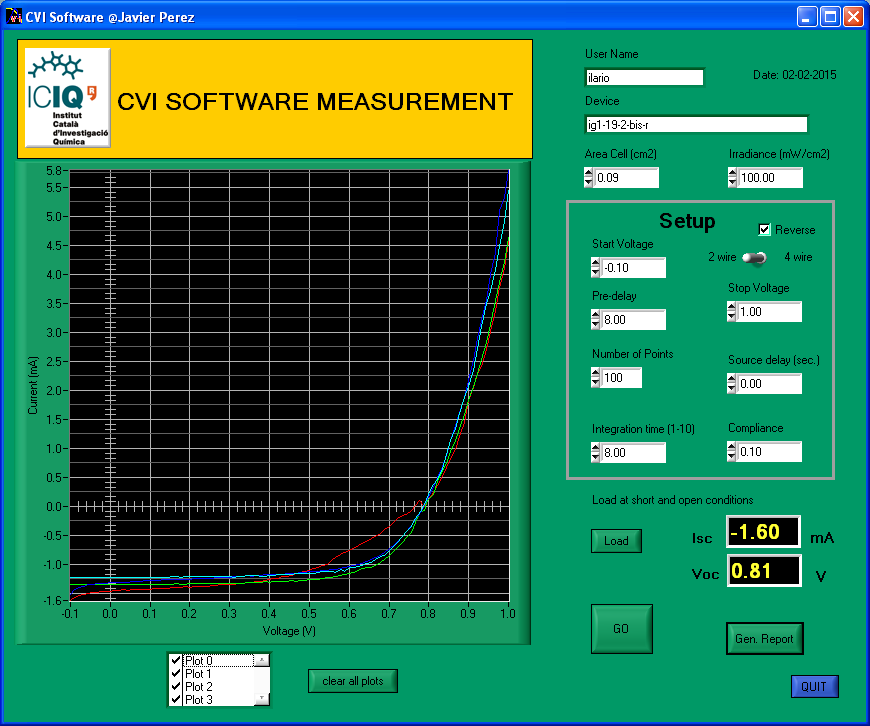
\includegraphics[width=0.7\textwidth]{old_iv_software/old_iv_software.png}
			\mycaption[Legacy software for current-voltage sweep measurement.]{}\label{fig:old_iv_software}
		\end{SCfigure}

		\paragraph{History of the project}
		As a proof of concept, Dr.\ Daniel Fernandez Pinto developed in 2015 a Python library and a small \gls{gui} for communicating with Tektronix Keithley 2400 equipment \textsl{via} NI-VISA \cite{NationalInstruments2019} and running basic operations like current\hyp{}voltage sweeps.
		I went on adding functions and expanding the \gls{gui} until obtaining a fully functional alternative to the legacy LabView software shown in \cref{fig:old_iv_software}.
		In comparison to the mentioned legacy software, PyPV has the advantage of not needing any commercial license which allowed us to use it on various computers.
		Additionally some of the features which will be described below were just missing in the previous software.
		As far as I know, PyPV is currently used in the following research institutions: ICIQ (Institut Català d’Investigació Química), URV (Universitat Rovira i Vrigili), İzmir Katip Çelebi Üniversitesi, and Karamanoglu Mehmetbey University.

		%I received a proof-of-concept software developed by  and decided to continue the development. At that point the software had an interface with few buttons and a working Keithley communication library.

		\paragraph{User's requests}
		The feedback from the new users of the software helped me improving PyPV in the following fields: solar simulator shutter control, more robust connection to the GPIB-USB-HS adapter, better installation instructions.

	\subsection{Implementation and user interface}
		\epigraph{\textit{\enquote{Ok, I finally completed it, by the way, why did you start developing this?}\\\enquote{Well, it was just a proof of concept, but it's nice you worked on it}}}

		Python~2, rather than the most recent Python~3, has been chosen for the software development.
		This apparently stupid choice was motivated by the requirement of running the software on the obsolete Windows~XP machines still used for the data acquisition.
		
		\begin{sidewaysfigure}
								\centering
			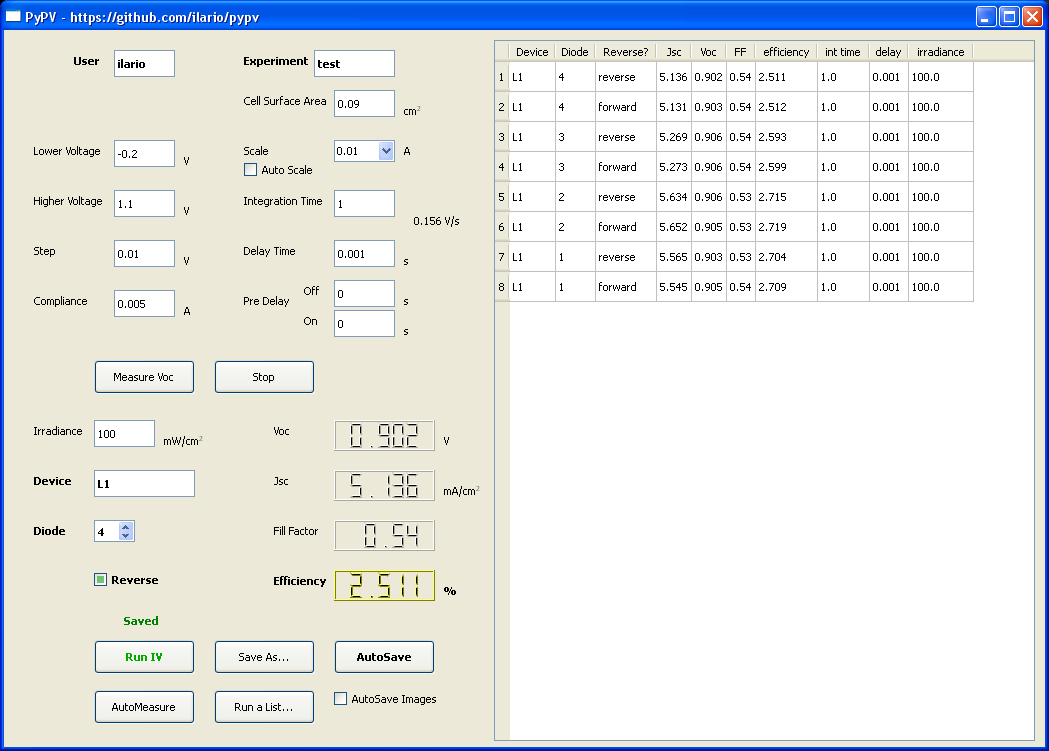
\includegraphics[width=0.9\textwidth]{PyPV/pypv-gui.png}
			\mycaption[PyPV graphical user interface.]{}\label{fig:pypv-gui}
		\end{sidewaysfigure}

%		\begin{landscape}
%							\begin{figure}
%					\centering
%					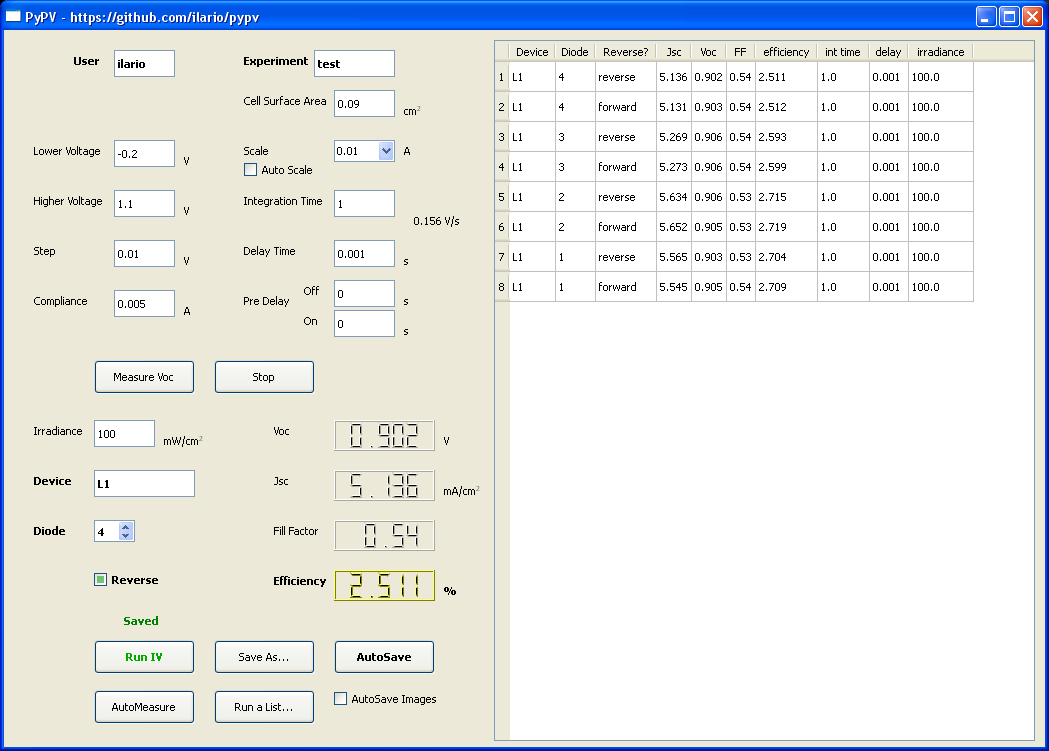
\includegraphics[width=1.1\textwidth]{PyPV/pypv-gui.png}
%					\mycaption[]{}\label{fig:pypv-gui}
%						\end{figure}
%		\end{landscape}

		
	
%		\begin{figure}
%			\makebox[\textwidth][c]{
%				\parbox{1.1\textwidth}{
%			\centering
%			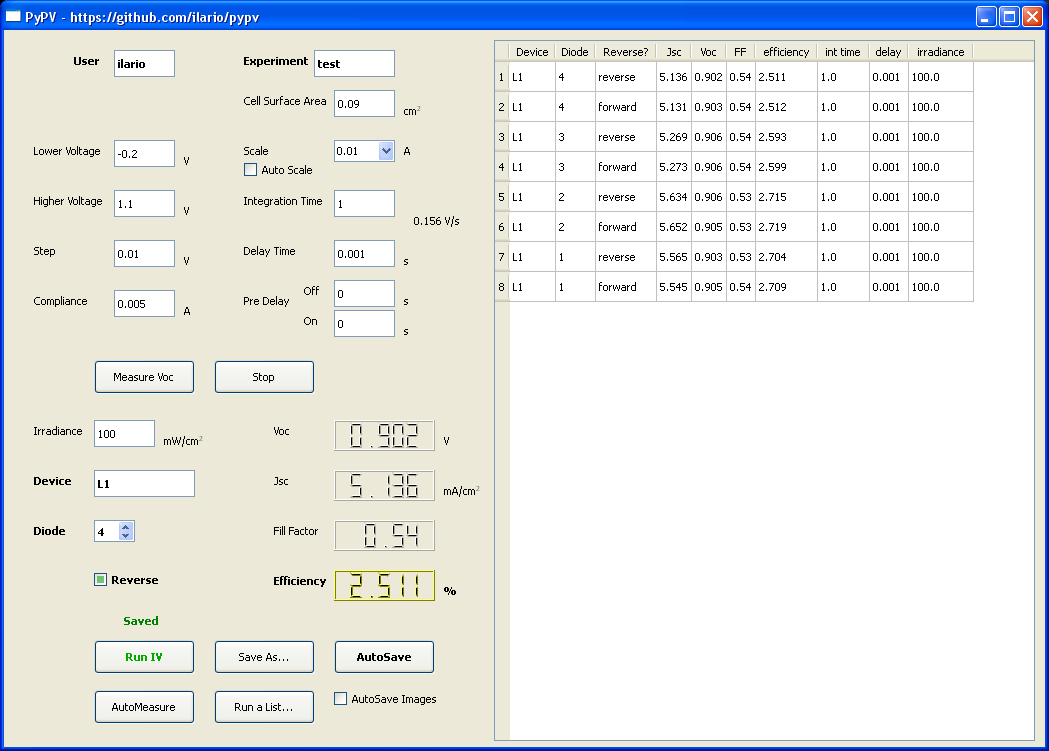
\includegraphics[width=1.1\textwidth]{PyPV/pypv-gui.png}
%			\mycaption[]{}\label{fig:pypv-gui}
%		}}
%		\end{figure}
		
		\paragraph{Autoscale} As it was explained in \cpageref{autoscale}, the automatic scale setting of the Keithley is detrimental for perovskite solar cells dynamic measurements.

		\paragraph{Auto-measure}\label{automeasure}
		The devices are kept under illumination at open circuit conditions, then a reverse sweep is measured and, immediately after this, the forward sweep is measured.
		The reason for measuring the reverse sweep first, is that the reverse sweep starts from a high voltage point which is closer to the stabilized condition of the devices prior to the measurement (illuminated and open circuit).


		\paragraph{Resistances} The shunt and series resistances estimation from current-voltage sweeps have been implemented but should not be considered for measurements on hysteretic devices, as explained in \cpageref{resistances}.

		\paragraph{Scan speed calculation}
		The scan speed $s[V/s]$ is obtained from the voltage step \texttt{:SENSe:VOLTage:STEP} $V_|step|[V]$, integration time \texttt{:SENSe:VOLTage:NPLCycles} $n_|int|$ measured in power line cycles and the delay time \texttt{:SOURce:DELay} $t_|delay|[s]$ Keithley's parameters with the following \textit{empirical} expression:

		\begin{equation}
			s = \frac{V_|step|}{0.003 + t_|delay| + 0.06 \cdot n_|int|}
		\end{equation}

		where $t_|delay|$ is \SI{1}{\ms} for our measurement conditions \cite{KeithleyInstruments2011}.

		\paragraph{Scan speed calculation}

\begin{SCfigure}
	\centering
	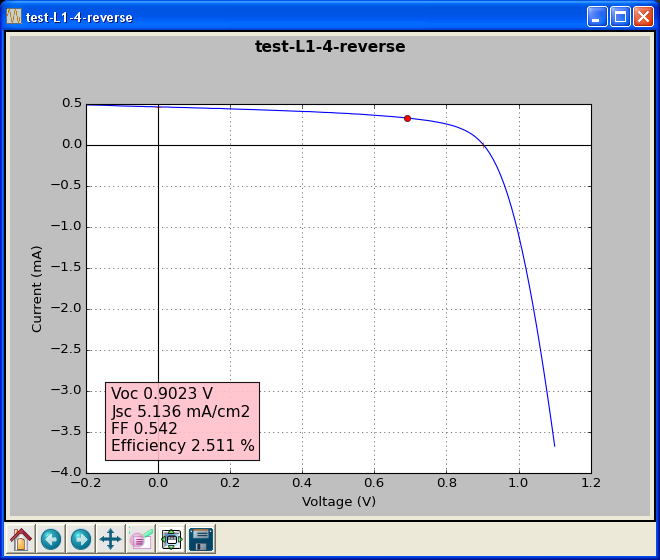
\includegraphics[width=0.7\textwidth]{PyPV/pypv-plot.png}
	\mycaption[]{}\label{fig:pypv-plot}
\end{SCfigure}

\paragraph{Additional output}

\begin{figure}
	\makebox[\textwidth][c]{
		\parbox{1.1\textwidth}{
			\centering
			\begin{subfigure}[t]{0.61\textwidth}
				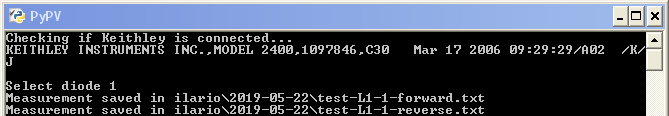
\includegraphics[width=1\textwidth]{PyPV/pypv-console.png}
				\subcaption{}\label{fig:pypv-console}
			\end{subfigure}
			\qquad
			\begin{subfigure}[t]{0.41\textwidth}
				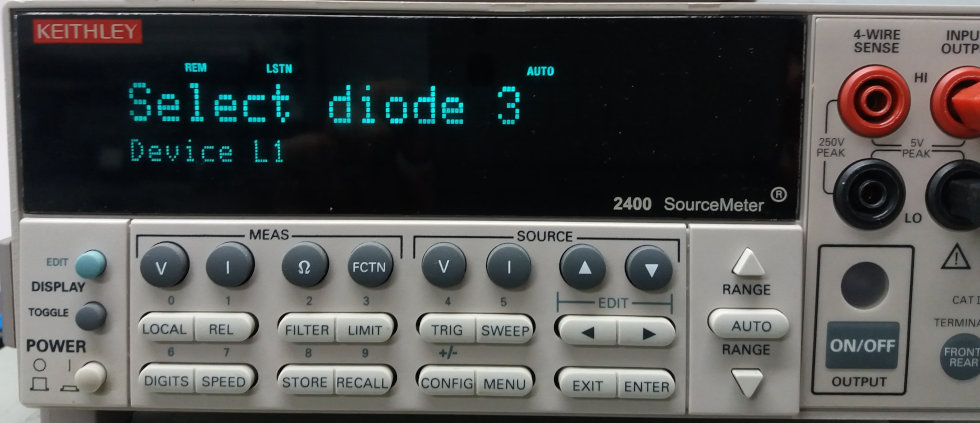
\includegraphics[width=1\textwidth]{PyPV/keithley.jpg}
				\subcaption{}\label{fig:pypv-keithley}
			\end{subfigure}
					\mycaption[]{}\label{fig:pypv-other}
		}
	}
\end{figure}

\paragraph{Last configuration saving}

	\subsection{Limitations}

		The interface development has been started with the "Monkey Studio" software, which development has ceased even before the start of PyPV. This demonstrated to be a big failure in long term development planning.

\pagebreak[2]
\section{Robust and quick data analysis \textsl{via} R scripts}
	\epigraph{\textit{\enquote{Is there an Origin version for Linux?}\\\enquote{No}}}

	\subsection{Introduction}
		To process the large amount of data which can be obtained using multiple techniques during the characterization of solar cells can be a very tedious and repetitive work.
		I developed routines for data processing and representation, like fittings, integrations and plots.
		I am describing the routines here in order to allow others to use and modify them.
		The described routines have been tested to work on Linux and Windows systems.
		All of the described functions can be downloaded from \url{https://github.com/ilario/photophysics-data-processing-R}.

	\subsection{Helpers}
		\paragraph{\texttt{limits\_for\_graphics.R} -- Set graphical parameters}
		In this file I tried to centralize the parameters which should be edited by the user and will be used by the scripts.
		This is for avoiding the need to edit "hardcoded" values in the middle of complex scripts.
		The parameters which can be customized here are: device active area, limits for the axes, string to prepend to the file names, switch between raster or vector image output, resolution of raster images output, size of vector image output.

		\paragraph{\texttt{devices-identification.R} -- Define grouping of devices}
		The devices are labelled with an alphanumeric codename, which is not insightful at the time of categorizing them for a statistical analysis.
		In this file the samples codes are grouped depending on one or two characteristics.
		Up to now, this system is just employed by \texttt{iv-generate\_mydata\_with\_comments.R} for adding supplementary information to the extracted parameters and by \texttt{iv-generate\_statistics.R} for plotting the boxplots separating the samples by kind.

		\paragraph{\texttt{run-all-photophysics.R} -- Runs routinely data analysis on one device's data}
		An extremely basic but multiplatform \gls{gui} has been implemented.
		Running it, the data folder gets prompted.
		By default, all the data analysis routinely performed in Palomares group is run.
		It can be edited to unselect the non-needed data analysis routines.
		
		\paragraph{\texttt{run-all-photophysics-comparisons.R} -- Plots comparisons between devices}
		This basic \gls{gui} prompts the user for the directories containing the data of each of the devices to be compared.
		Then it plots the characterization data of all the selected devices in single plots, in order to help the visual comparison of the results.
		
		%\subsection{Photophysical Characterization \textsl{via} Optical and Electrical Transients}


	\subsection{Charge Extraction (\glsentryshort{ce})}\label{r_ce}

		\paragraph{\texttt{from\_ce\_to\_table.R} -- Converts CE output}
		The output from \gls{ce} measurement software is rather minimal, as it lacks the time column.
		This script generates a two column file output which is more convenient for plotting with other commonly employed software.
		It works both for the TPV and for the TPC outputs.
		
		\paragraph{\texttt{ce.R} -- Integrates CE transients directly}
		\paragraph{\texttt{ce-subtractDark.R} -- Integrates CE transients after subtracting a transformed noise profile}
		\paragraph{\texttt{ce-integrateExp.R} -- Integrates a fit to CE transients}
		\paragraph{\texttt{ce-from\_output\_to\_graph.R} -- Plots the extracted charge \textsl{versus} light bias}
		\paragraph{\texttt{ce-from\_many\_output\_to\_graph.R} -- Compares between CE of various devices}
		\paragraph{\texttt{ce-time-many.R} -- Compares single CE transients of various devices}
		\paragraph{\texttt{ce-with\_limits.R} -- Compares CE transients with RC decays}

	\subsection{Transient PhotoVoltage (\glsentryshort{tpv})}\label{r_tpv}

		\paragraph{\texttt{from\_tpv\_tpc\_to\_table.R} -- Converts CE output}
		Similarly to \texttt{from\_ce\_to\_table.R}, this converts the one column raw file to a two columns text file.

		\paragraph{\texttt{tpv.R} -- Fits TPV decays}
		
				\paragraph{\texttt{tpv\_onlyDeltaV.R} -- Gets the voltage increase from TPV decays}
				
		\paragraph{\texttt{tpv-from\_output\_to\_graph.R} -- Plots TPV life\hyp{}times \textsl{versus} light bias}
		
		
\paragraph{\texttt{tpv-from\_output\_to\_graph-with\_limits.R} -- Compares life\hyp{}time with RC time}

		\paragraph{\texttt{tpv-from\_many\_output\_to\_graph.R} -- Compares between TPV of various devices}

	\subsection{Transient PhotoCurrent (\glsentryshort{tpc})}\label{r_tpc}

		\paragraph{\texttt{tpc.R} -- Integrates TPC transients}
		\paragraph{\texttt{tpc-vs-tpv-vs-ce.R} -- Compares the single transients from various techniques}


	\subsection{Differential Capacitance (\glsentryshort{dc})}\label{r_dc}

		\paragraph{\texttt{dc-from\_output\_to\_graph.R} -- Calculates and plots capacitance and charge from DC}
		
		\paragraph{\texttt{cedc.R} -- Compares the charge \textsl{versus} light\hyp{}bias obtained from CE or DC}
		
		\paragraph{\texttt{dc-from\_many\_output\_to\_graph\_capacitance.R} and \texttt{dc-from\_many\_output\_to\_graph\_charge.R} -- Compares between DC of various devices}
		

	\subsection{Transient PhotoVoltage referred to charge from CE or DC (\glsentryshort{tpvce} and \glsentryshort{tpvdc})}\label{r_tpvcedc}



		\paragraph{\texttt{tpvce-from\_output\_to\_graph.R} -- Relate TPV life\hyp{}times to CE charge}
		
				\paragraph{\texttt{tpvce-from\_many\_output\_to\_graph.R} and \texttt{tpvdc-from\_many\_output\_to\_graph.R} -- Compare TPV life\hyp{}times related to either CE or DC charge of various devices}

	\subsection{Current-Voltage Sweeps}
		\paragraph{\texttt{extractdata-curves-vi-separated\_files.R} -- Functions for extracting parameters from current\hyp{}voltage sweeps¨}
		\paragraph{\texttt{iv-generate\_mydata.R} and \texttt{iv-generate\_mydata\_with\_comments.R}}
		\paragraph{\texttt{iv-generate\_images.R}}
		\paragraph{\texttt{iv-generate\_statistics.R}}
		\paragraph{\texttt{iv-jsc\_voc\_vs\_light\_intensity.R}}
		\paragraph{\texttt{iv-plot\_list.R}, \texttt{iv-plot\_list-suppinfo.R}, and \texttt{iv-light\_intensity.R}}

		\paragraph{\texttt{jsc-stability.R} and \texttt{voc-stability.R}}

	\subsection{Other}
	
				\paragraph{\texttt{jrec-ce.R} and \texttt{jrec-dc.R} -- Reconstructs the \gls{jsc}}
					\cpageref{jsc_reconstruction}
					
		\paragraph{\texttt{mppt\_to\_graph.R} -- Plots tracking of maximum power point}
		\paragraph{\texttt{profilometry.R} -- Plots profilometer measurements and fit heights}
		\paragraph{\texttt{tas-downsample.R} -- Reduces the dimension of TAS decays}
%		\paragraph{\texttt{tas-graph.R} -- Plots TAS decays}
		\paragraph{\texttt{uvvis-pl.R} -- Plots absorbance and photoluminescence spectra and fits Tauc plots}

\section{Contributions to mppTracker}\label{software_mppt}
	\epigraph{\textit{\enquote{A student of mine sells a complete system for that, just go and buy it}}}

	As seen in \cpageref{characterization_hysteresis}, a \gls{mppt} system ensures to obtain a \gls{pce} value closer to the real world working conditions.
	The hysteretic phenomena in perovskite solar cells requires new procedures for \gls{mppt} \cite{Cimaroli2017,Pellet2017} and a few commercial systems are already available for that \cite{CicciResearchsrl2019,CandlelightSystems}.
	An interesting project for having robust \gls{mppt} measurable with Tektronix Keithley 2400 is mppTracker \cite{AFMD2017}.
	I made a few contributions which are accessible on \url{https://github.com/AFMD/mppTracker/pulls?q=is%3Apr}.
	As the effort in this project were very limited on my side, I'll not further describe that.
	If confirmed, recent reports on "bistable short circuit current" in perovskite solar cells by \authoryear{Calado2018} would further complicate the implementation of a \gls{mppt}.
%	introduce local maxima making the \gls{mppt} system design even more complex.
